\chapter{Evaluation}
\label{chapter:evaluation}

\section{A Performance Evaluation of the SFM-LSD Pipeline at 100m Altitude}\label{sec:sfm_lsd_eval}
\section{Experimental Setup}

The pipeline was tested by repeatedly flying a mission with randomized initial conditions.

The performed experiments were flown on the following two maps:
\begin{itemize}
    \item Arroyo Map - Prerecorded Gazebo map from the Arroyo Seco area outside the East entrance of the Jet Propulsion Laboratory.
    \begin{figure}[h]
        \centering
        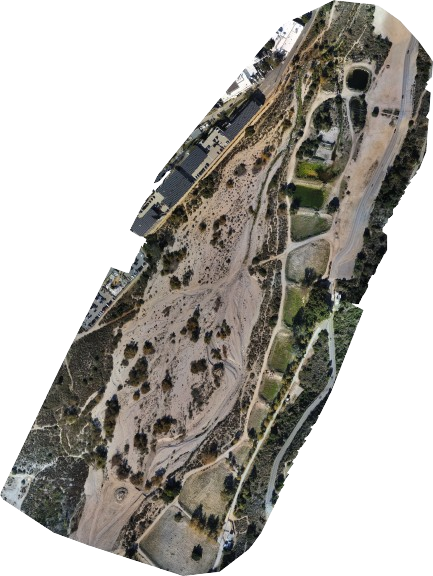
\includegraphics[scale=0.5]{images/evaluation/arroyo.png}
        \caption{Map of the Arroyo Seco area outside of the Jet Propulsion Laboratory}
    \end{figure}
    \begin{figure}[h]
        \centering
        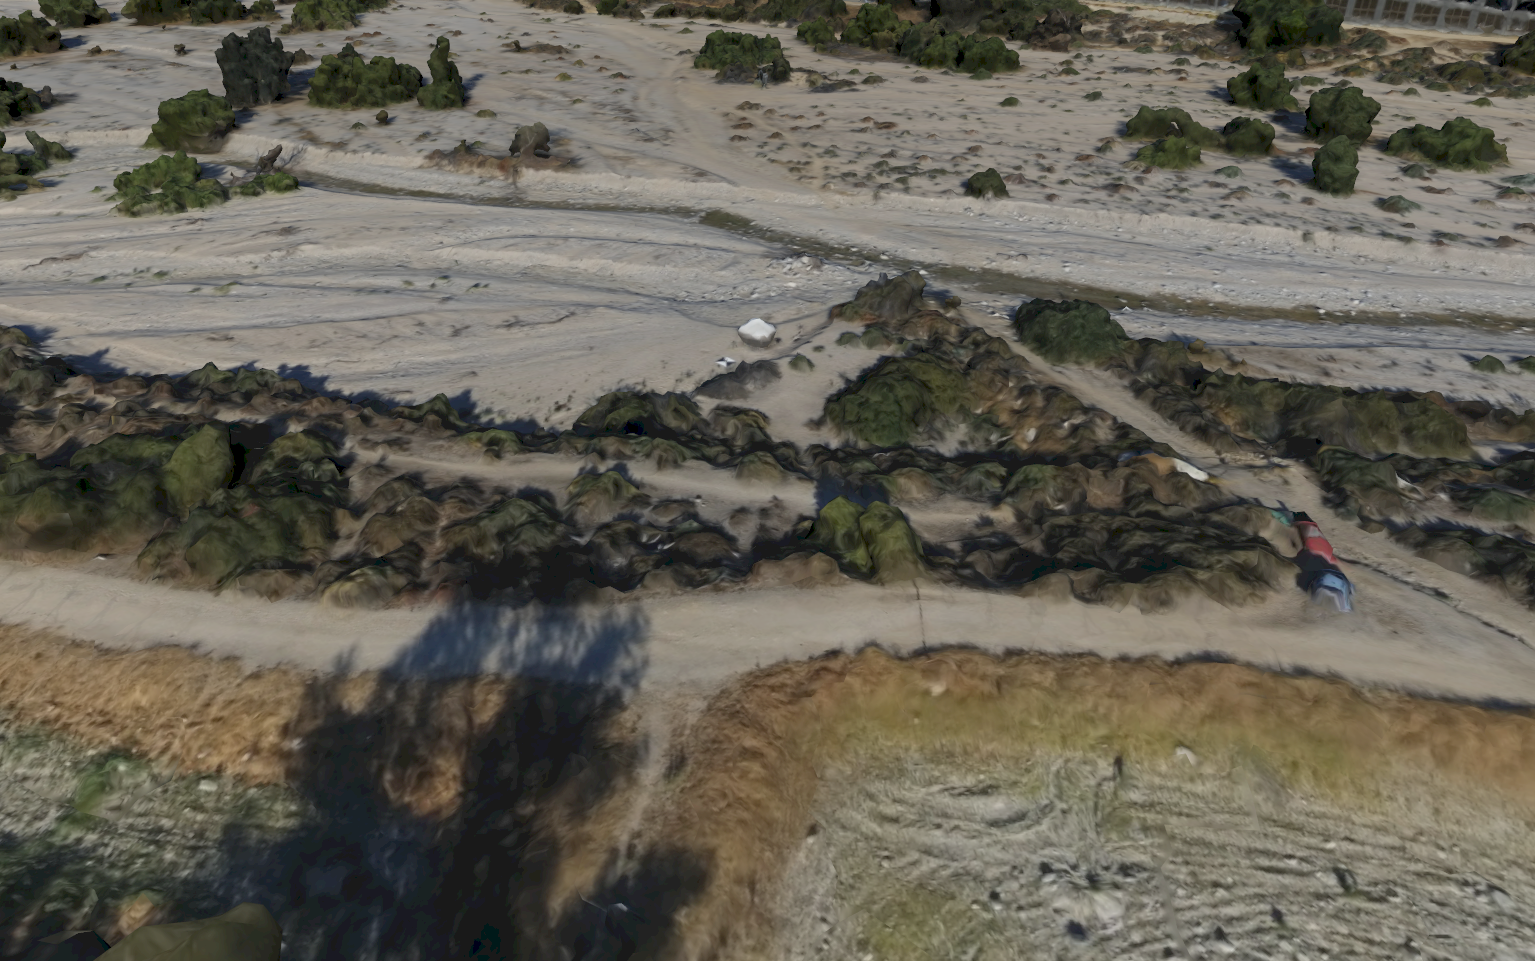
\includegraphics[scale=0.23]{images/evaluation/arroyo_map.png}
        \caption{Close Up of the Arroyo Map}
    \end{figure}
    \item Rough Test Map - A control environment designed to prevent LSD from detecting any landing site unless a landing platform is specifically spawned. 
    \begin{figure}[h]
        \centering
        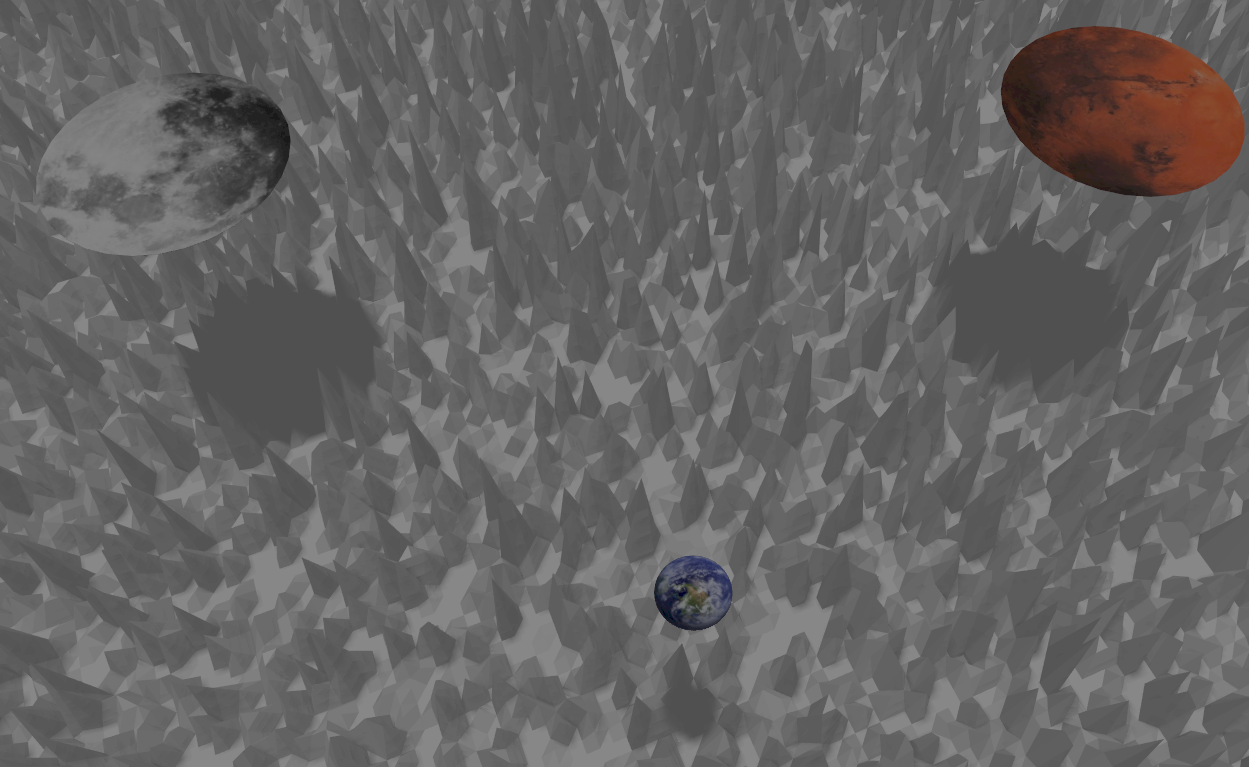
\includegraphics[scale=0.285]{images/evaluation/rough_test_map.png}
        \caption{Synthetically created map with no landing sites apart from inserted landing platforms.}
    \end{figure}
    \begin{figure}[h]
        \centering
        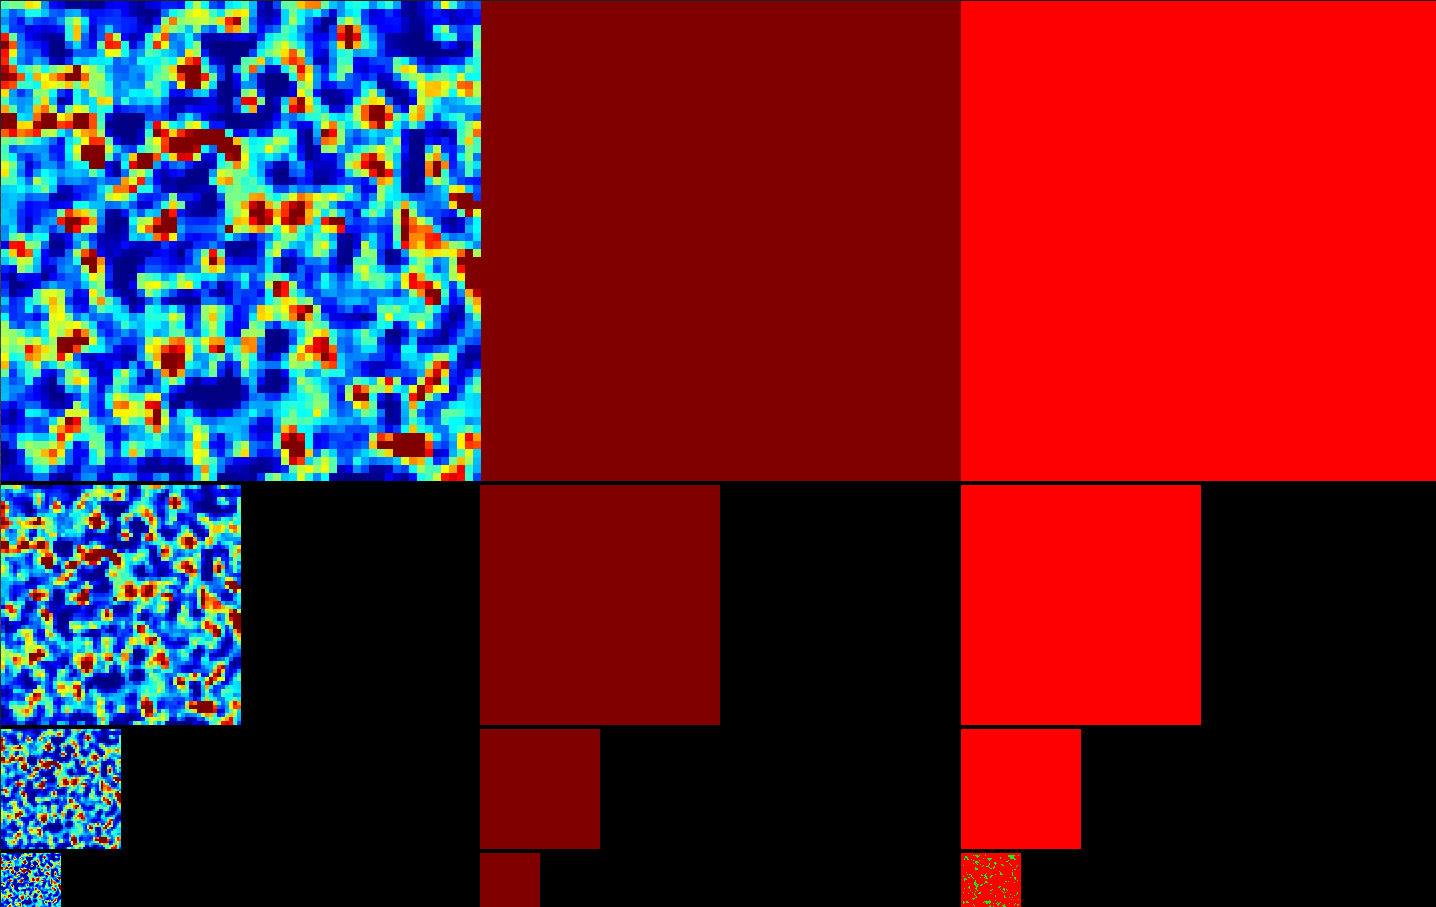
\includegraphics[scale=0.25]{images/evaluation/rough_map_LSD.png}
        \caption{LSD debug output shown of the plain rough environment}
    \end{figure}
    \begin{figure}[h]
        \centering
        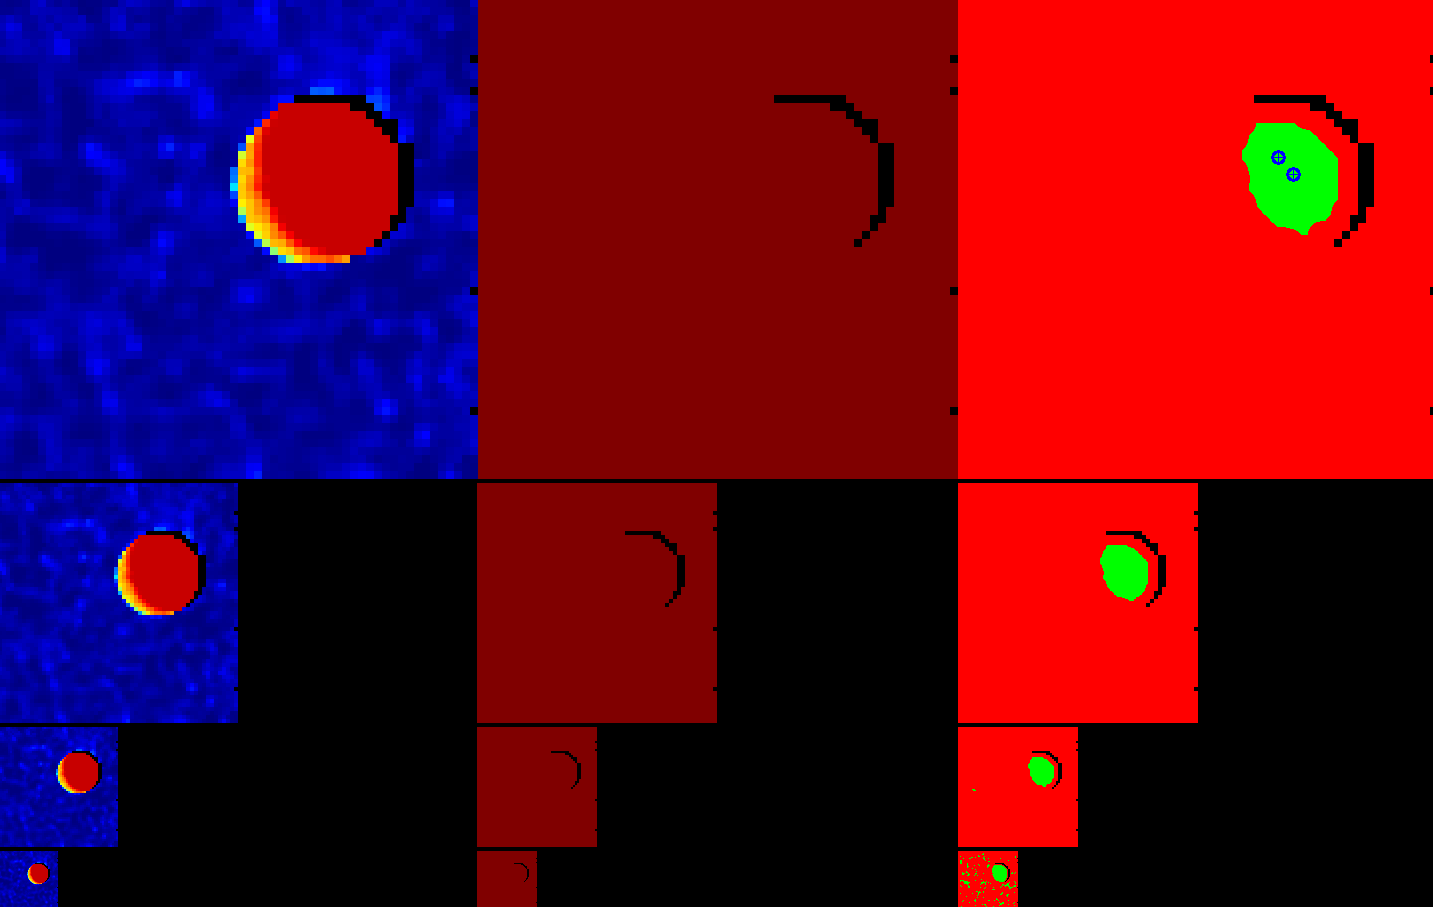
\includegraphics[scale=0.25]{images/evaluation/rough_map_LSD_platform.png}
        \caption{LSD debug image of the rough control map with spawned landing platforms}
    \end{figure}
\end{itemize}
\clearpage %HERE
\subsection{Drone Spawn}
The drone was either spawned repetetively from a default location on the ground (The start location from when the actual fields tests were performed) or from a random location. For a simplicity way of  avoiding terrain collisions, the drone was spawned on a randomly positioned disk at 40m altitude. The start disk's size was only 0.5m in diameter which prevented it from being considered too good of a landing site by LSD. This is important because the platform implicitly gains quality due to the fact, that it is located higher up than the terrain, leading to a lower distance to the drone when flying at mission altitude.
\begin{figure}[h]
    \centering
    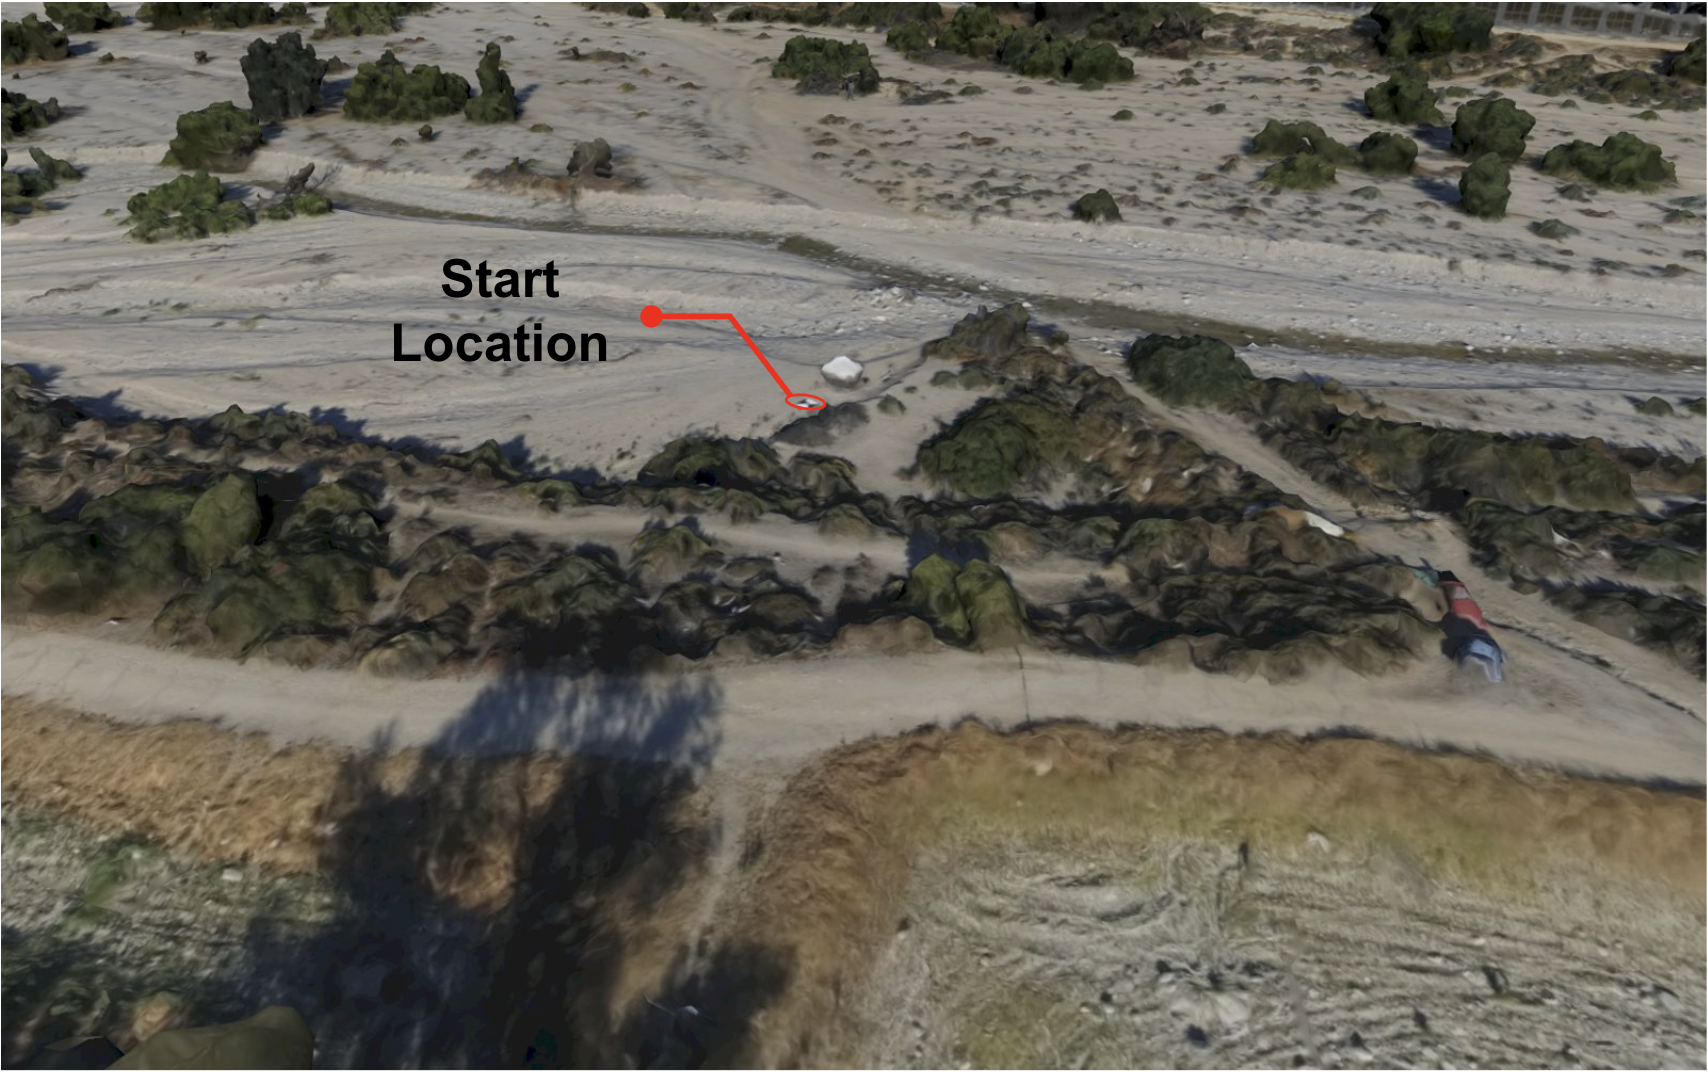
\includegraphics[scale=0.42]{images/evaluation/arroyo_with_start.png}
    \caption{Arroyo Map with Fixed Start Position}
    \label{fig:fixed_start}
\end{figure}
\begin{figure}[h]
    \centering
    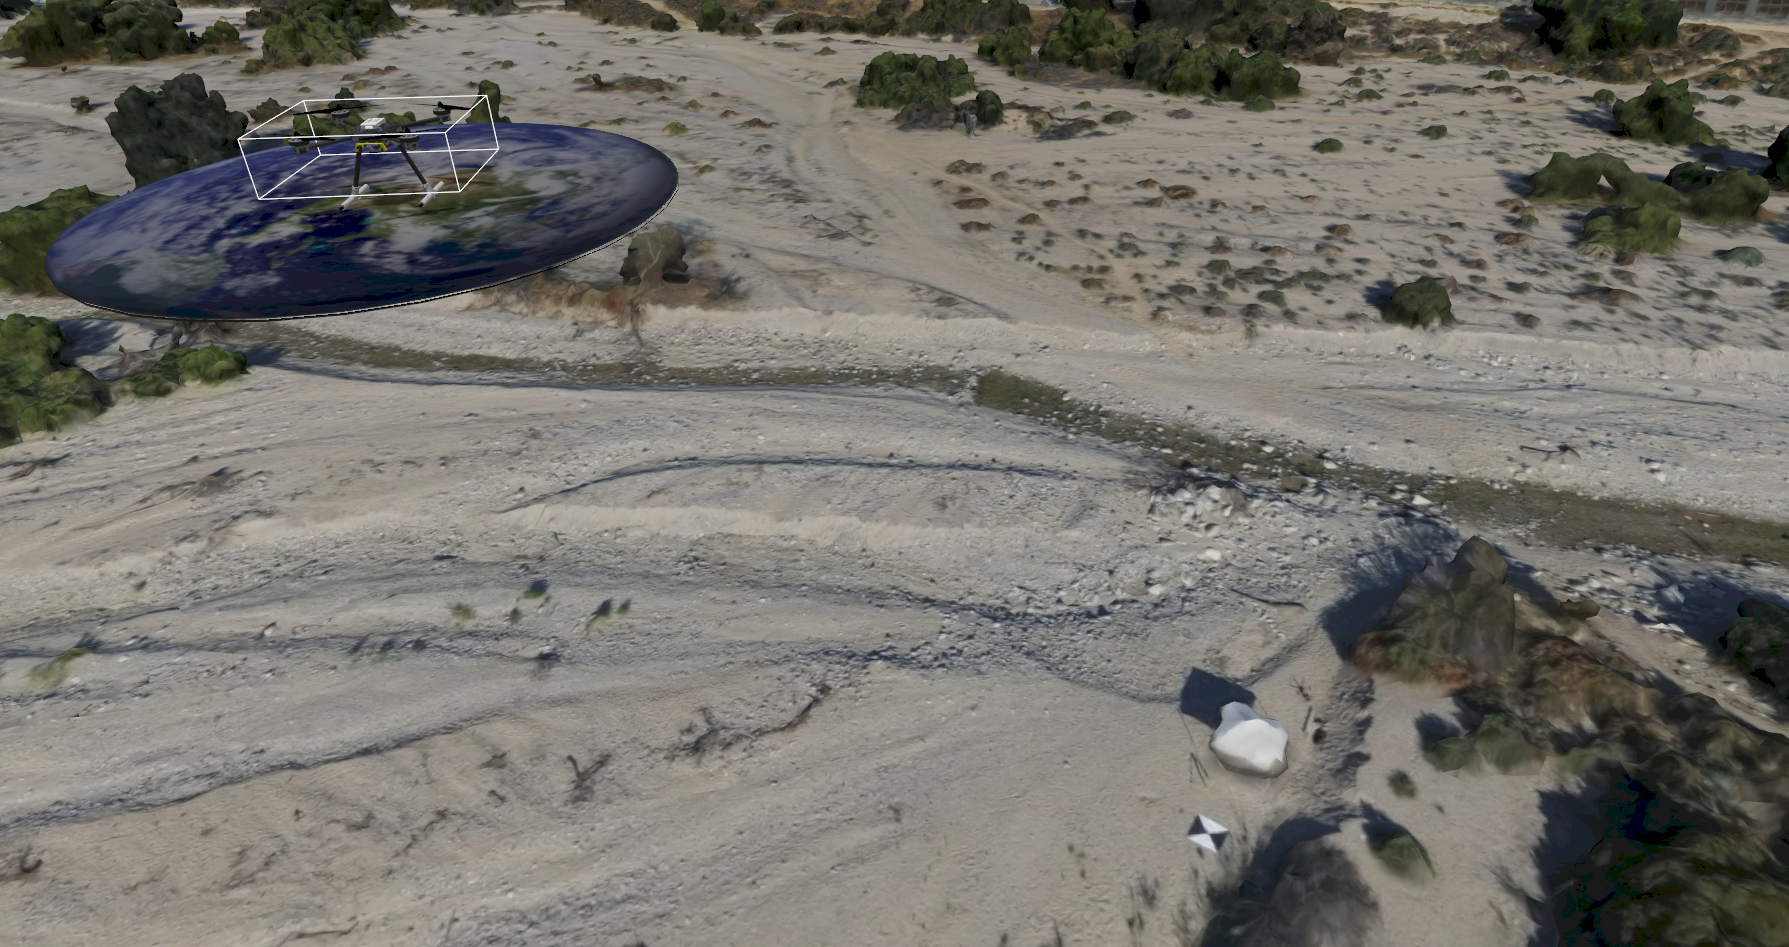
\includegraphics[scale=0.2]{images/evaluation/arroyo_with_platform.png}
    \caption{Arroyo map with randomly positioned spawn platform}
    \label{fig:random_start}
\end{figure}
\clearpage %HERE

\subsection{Depth Source}
As mentioned in \cref{sec:sfm_lsd_eval}, at the time of this work SFM was very fragile as an individual module. Because of this and to evaluate the built pipeline as opposed to the depth generation module, ground truth depth was used at high altitudes unless specified otherwise. Regardless of whether ground truth or SFM was used, the verification at low altitudes was always performed using the point clouds from the stereo camera depth node.

\subsection{Success Conditions}
To determine whether a flight was successful or not, two main metrics were considered. First of all whether the landing action in the autonomy was initiated (this happens only after the landing site selection and verification were both successful) and secondly to infere the safety of the rotorcraft, a rosbag was collected and analyzed to check whether either the roll or pitch value exceeded the crash threshold.

\textbf{Note: } In practice a threshold of 1.2 radians or shortly below 70\degree proved to be an accurate decision boundary.

\subsection{Visual Analysis}
To further analyze the randomized flights in a bit more detail, visual landing attempt projections are used:

\begin{figure}[h]
    \begin{center}
        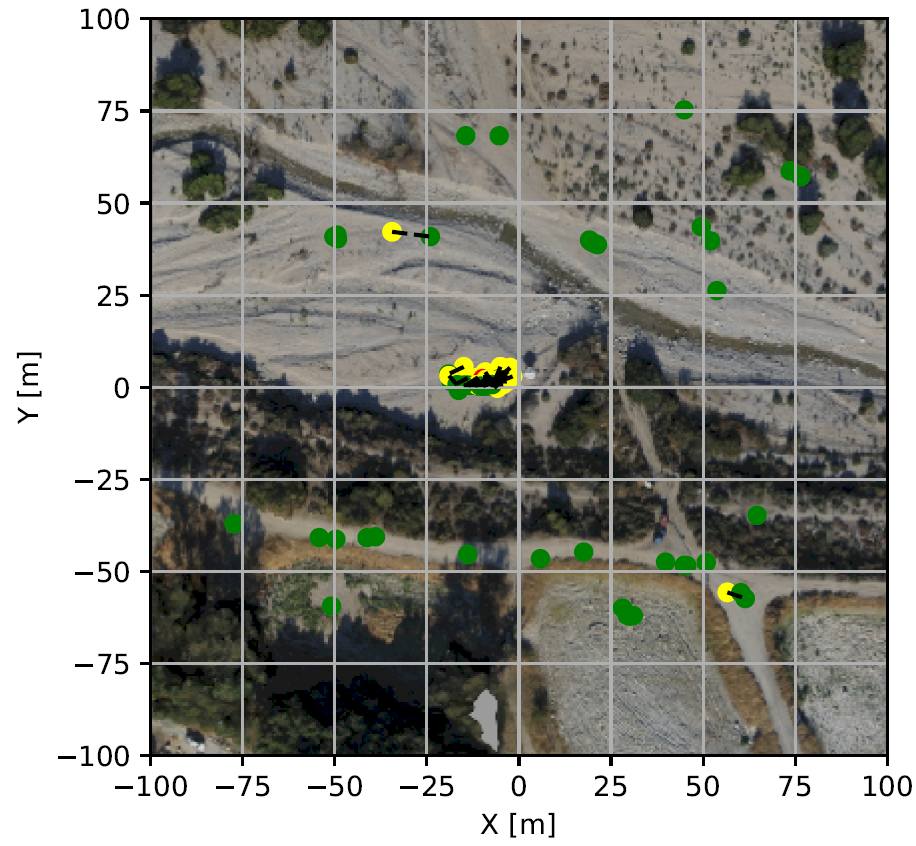
\includegraphics[scale=0.25]{images/evaluation/landings_random_WP_GT.png}
        \caption{Landing Attempt dummy image - Green: successful landing, Yellow: verification failure, Blue: landing at home position}
        \label{fig:landing_attempts_dummy}
    \end{center}
\end{figure}

The green points indicate successful verifications which lead to the initiation of the landing action shortly after. (If no rotation above a failure threshold was detected, this is considered a success.) 

The yellow points are landing attempts, where a chosen landing site was not verified and thus banned from further consideration. It is crucial to note that this is perfectly correct behavior. Landing sites detected at high altitudes merely provide a preliminary indication of potential landing zones.  It is the subsequent phase, responsible for verifying these sites, that identifies the most promising areas for landing. So selecting a landing site, attempting to verify it but failing to do so and subsequently choosing a close by landing site detected at this low verification altitude might even be called the most promising chain of actions in the pursuit of autonomous landing.

Lastly, blue points indicate successful landings at the home position. When flying on a map with obvious landing opportunities, landing at the home position indicates an issue with the landing site detection mechanism. This is because the rotorcraft will only settle at the home position if no other landing site, regardless of quality, is currently available and the maximum number of additional landing site search excursions%TODO: add reference to the Schlenker
 has been performed.

\subsection{Offboard Mode connection Issues}
As will be presented in the following, connection failures between the PX4 flight controller and the autonomy ocurred, leading to the deactivation of the offboard mode and therefore the loss of control of the autonomy over the rotorcraft. These issues arose most likely because the mavros connection inbetween failed to send a necessary heartbeat repeatedly and thus the connection was intercepted.

Self evidently, this did not result in a successful landing and was not counted as such. However, as these connection issues did not occur due to insufficiencies in the pipeline presented in this work, they were not considered failures of the pipeline either.
\clearpage
\section{Test Flights}
\subsection{Arroyo - Randomized Waypoints}

When starting 100 times from the fixed position indicated in \cref{fig:fixed_start} and flying to random mission waypoints at 100m altitude in a 70x70m vicinity on the Arroyo map, the following results were achieved:

\begin{table}[h]
    \begin{center}
     \caption{Results with fixed takeoff and random waypoint}\vspace{1ex}
     \label{tab:result_random_waypoint}
     \begin{tabular}{|c|c|c|c|c|}
     \hline
     \# Flights & \# Successes & \# Timeouts & \# Crashes & \# Home Landing\\ \hline \hline
     100 & 97 & 3 & 0 & 0 \\%TODO: replace with correct values
     \hline
     \end{tabular}
    \end{center}
    \end{table}

    The landing attempt numerics are shown here:
    \begin{table}[h]
        \begin{center}
         \caption{Landing attempts with fixed takeoff and random waypoint}\vspace{1ex}
         \label{tab:land_nums_random_waypoint}
         \begin{tabular}{|c|c|c|c|}
         \hline
         \# Flights & \# Landing on first attempt & \# 2 attempts & \# 3 attempts\\ \hline \hline
         100 & 50 & 47 & 3 \\%TODO: replace with correct values
         \hline
         \end{tabular}
        \end{center}
    \end{table}

    \begin{figure}[h]
        \begin{center}
            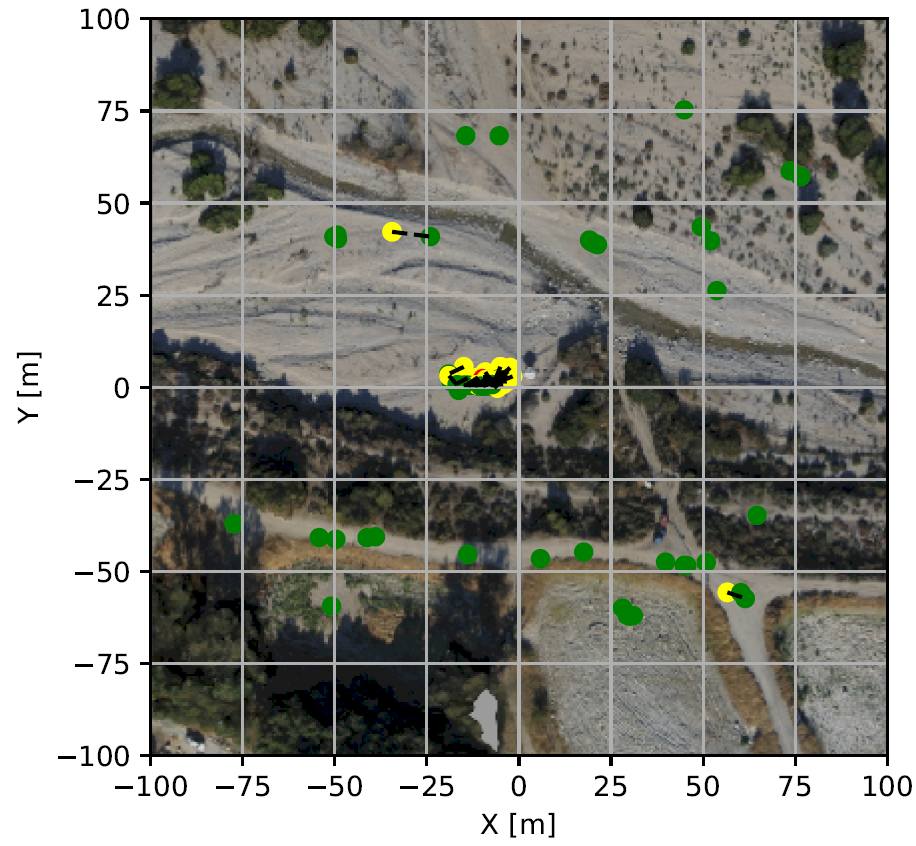
\includegraphics[scale=0.25]{images/evaluation/landings_random_WP_GT.png}
            \caption{Landing Attempts - Green: successful landing, Yellow: verification failure, Blue: landing at home position}
            \label{fig:landing_attempts_random_WP}
        \end{center}
    \end{figure}%TODO replace with new one

    \subsubsection{Numeric Discussion}
    \cref{tab:result_random_waypoint} shows the numeric outcome of the flights. 3 timeouts ocurred but each performed flight by the autonomy was a success, landing safely and controlled. No home landings were necessary which, as described above, indicates a very robust LSD performance. 

    \subsubsection{Visual Discussion}
    Let's consider the landing image \ref{fig:landing_attempts_random_WP}. Though hard to see, the final landing sites indicated in green span exclusively decent landing areas. The verification attempts that fell short are indicated with yellow. The first detail to emphasize on is the proximity of yellow points to green ones. This is also a desirable characteristic as the drone should not waste time pursuing a far away landing site when failing a verification. As indicated in \cref{subsubsec:ver_alt} this is thanks to the verification altitude which incentivises the selection of other landing sites detected at the current verification altitude.

    The last thing to mention is the clustering of the landing sites around the takeoff location. The reason for this is twofold:
    \begin{itemize}
        \item \textbf{Quality}: The takeoff position was the also the takeoff position for the physical flights in performed in the field. It was chosen exactly because of its even and smooth characteristics. Therefore it is no surprise that many landing sites were detected around that location.
        \item \textbf{OMG Conversion}: During ascent, when using either stereo or ground truth depth, the same area is perceived repeatedly. This leads to a convergence in certainty in the map aggregation step of LSD. As landing sites have a higher chance of being detected on terrain with a low uncertainty, the takeoff position is mostl likely selected until it leaves the rolling buffer map.
    \end{itemize}

    This test is a very clear demonstration of the applied chosen heuristics. The best landing site detected is very likely one that is detected at the takeoff position. Around this clustering of landings there is notable space of no attempts performed. This can be attributed to the competing motives of the landing site selection. The quality of the landing site defines the autonomy's choice until the drone's distance to that landing site is too big and a closer one is chosen. 

    \subsection{Arroyo - Randomized Takeoff and Waypoints}

    In this set of test flights, randomized takeoff positions were used as shown in \cref{fig:random_start}. Missions were built using a randomized waypoint in a 70x70m surrounding.

    The numerical results look as follows:

    \begin{table}[h]
        \begin{center}
         \caption{Results with random takeoff location and random waypoint}\vspace{1ex}
         \label{tab:result_complete_rand}
         \begin{tabular}{|c|c|c|c|c|}
         \hline
         \# Flights & \# Successes & \# Timeouts & \# Crashes & \# Home Landing\\ \hline \hline
         100 & 97 & 3 & 0 & 0 \\%TODO: replace with correct values
         \hline
         \end{tabular}
        \end{center}
    \end{table}
    \begin{table}[h]
        \begin{center}
         \caption{Landing attempts with random takeoff and random waypoint}\vspace{1ex}
         \label{tab:land_nums_complete_rand}
         \begin{tabular}{|c|c|c|c|}
         \hline
         \# Flights & \# Landing on first attempt & \# 2 attempts & \# 3 attempts\\ \hline \hline
         100 & 50 & 47 & 3 \\%TODO: replace with correct values
         \hline
         \end{tabular}
        \end{center}
    \end{table}

    And the visual outcome:

    \begin{figure}[h]
        \begin{center}
            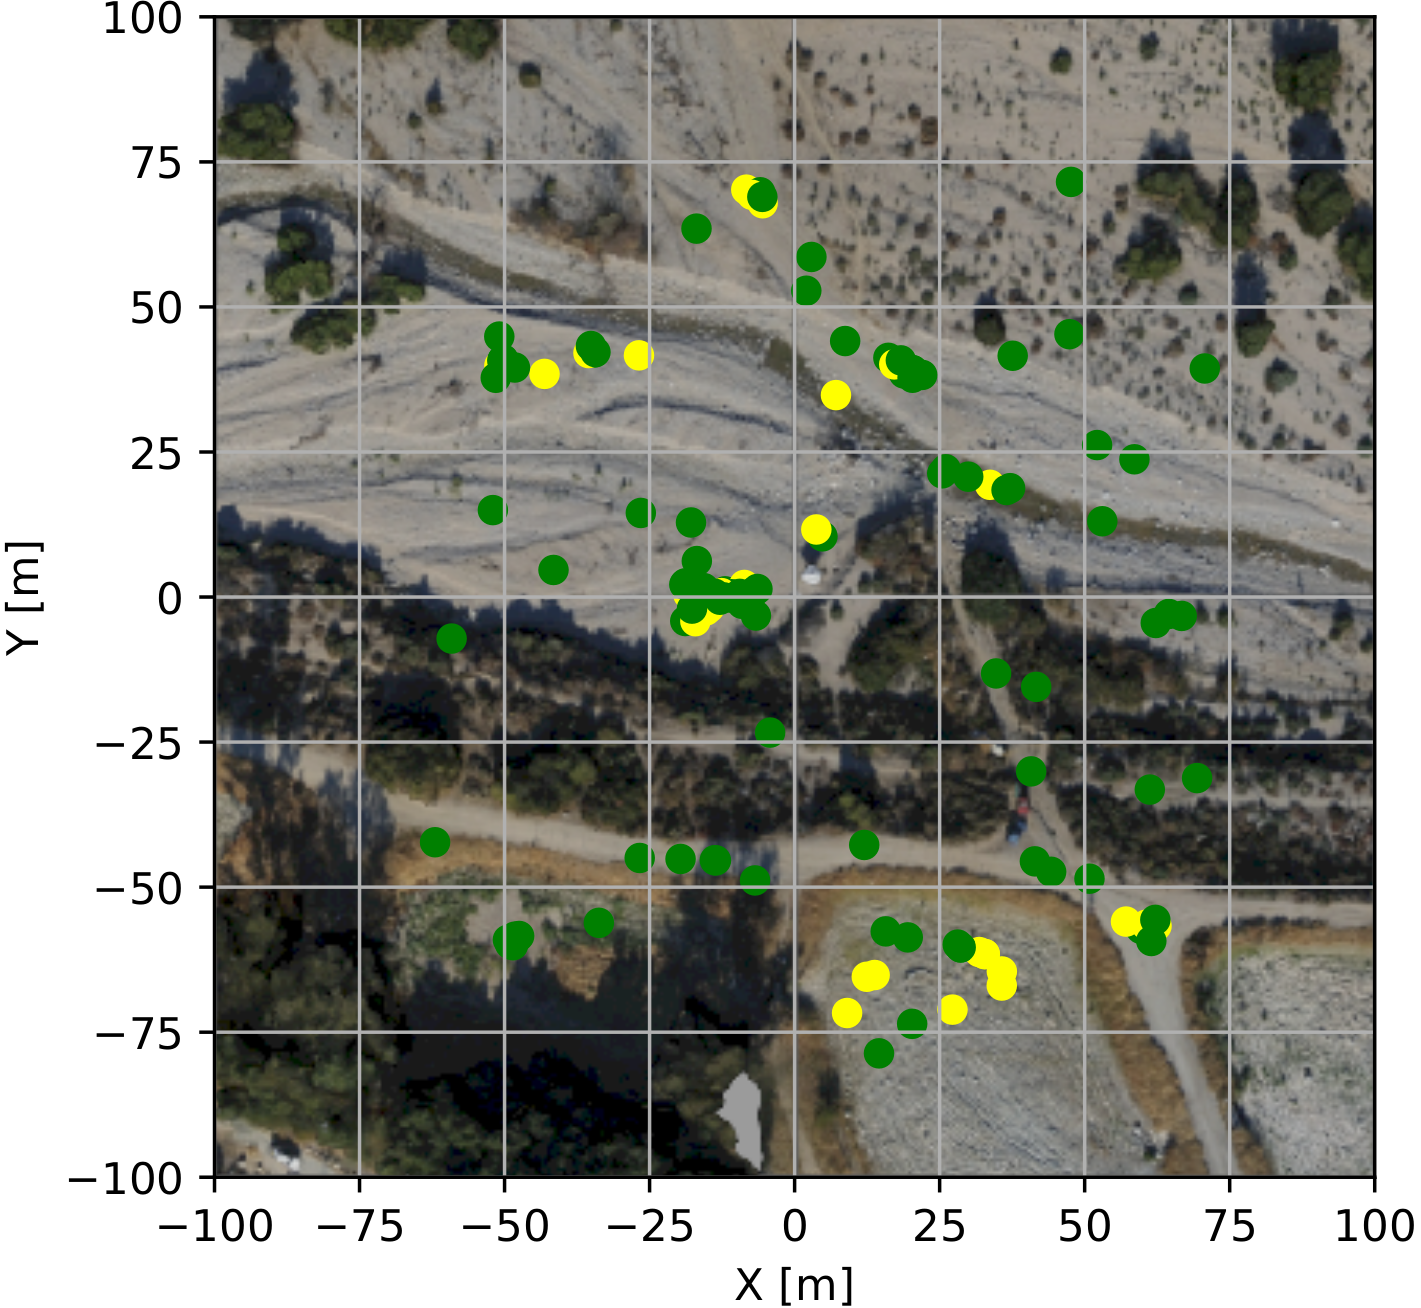
\includegraphics[scale=0.25]{images/evaluation/landings_complete_randomized_GT.png}
            \caption{Landing Attempts - Green: successful landing, Yellow: verification failure, Blue: landing at home position}
            \label{fig:landing_attempts_complete_rand}
        \end{center}
    \end{figure}%TODO replace with new one

    \subsubsection{Numeric Discussion}



    \subsubsection{Visual Discussion}
    Compared to \cref{fig:landing_attempts_random_WP}, the landing attempts are more spread out over the map. Fewer landings were attempted at the takeoff position. This is the case because the area wasn't always covered by the mission's trajectory and the pipeline very probably did not converge at that location.

    \subsection{Rough Map - Random Waypoints over Platforms}\label{subsec:rough_coverage}
        \begin{figure}[h]
            \centering
            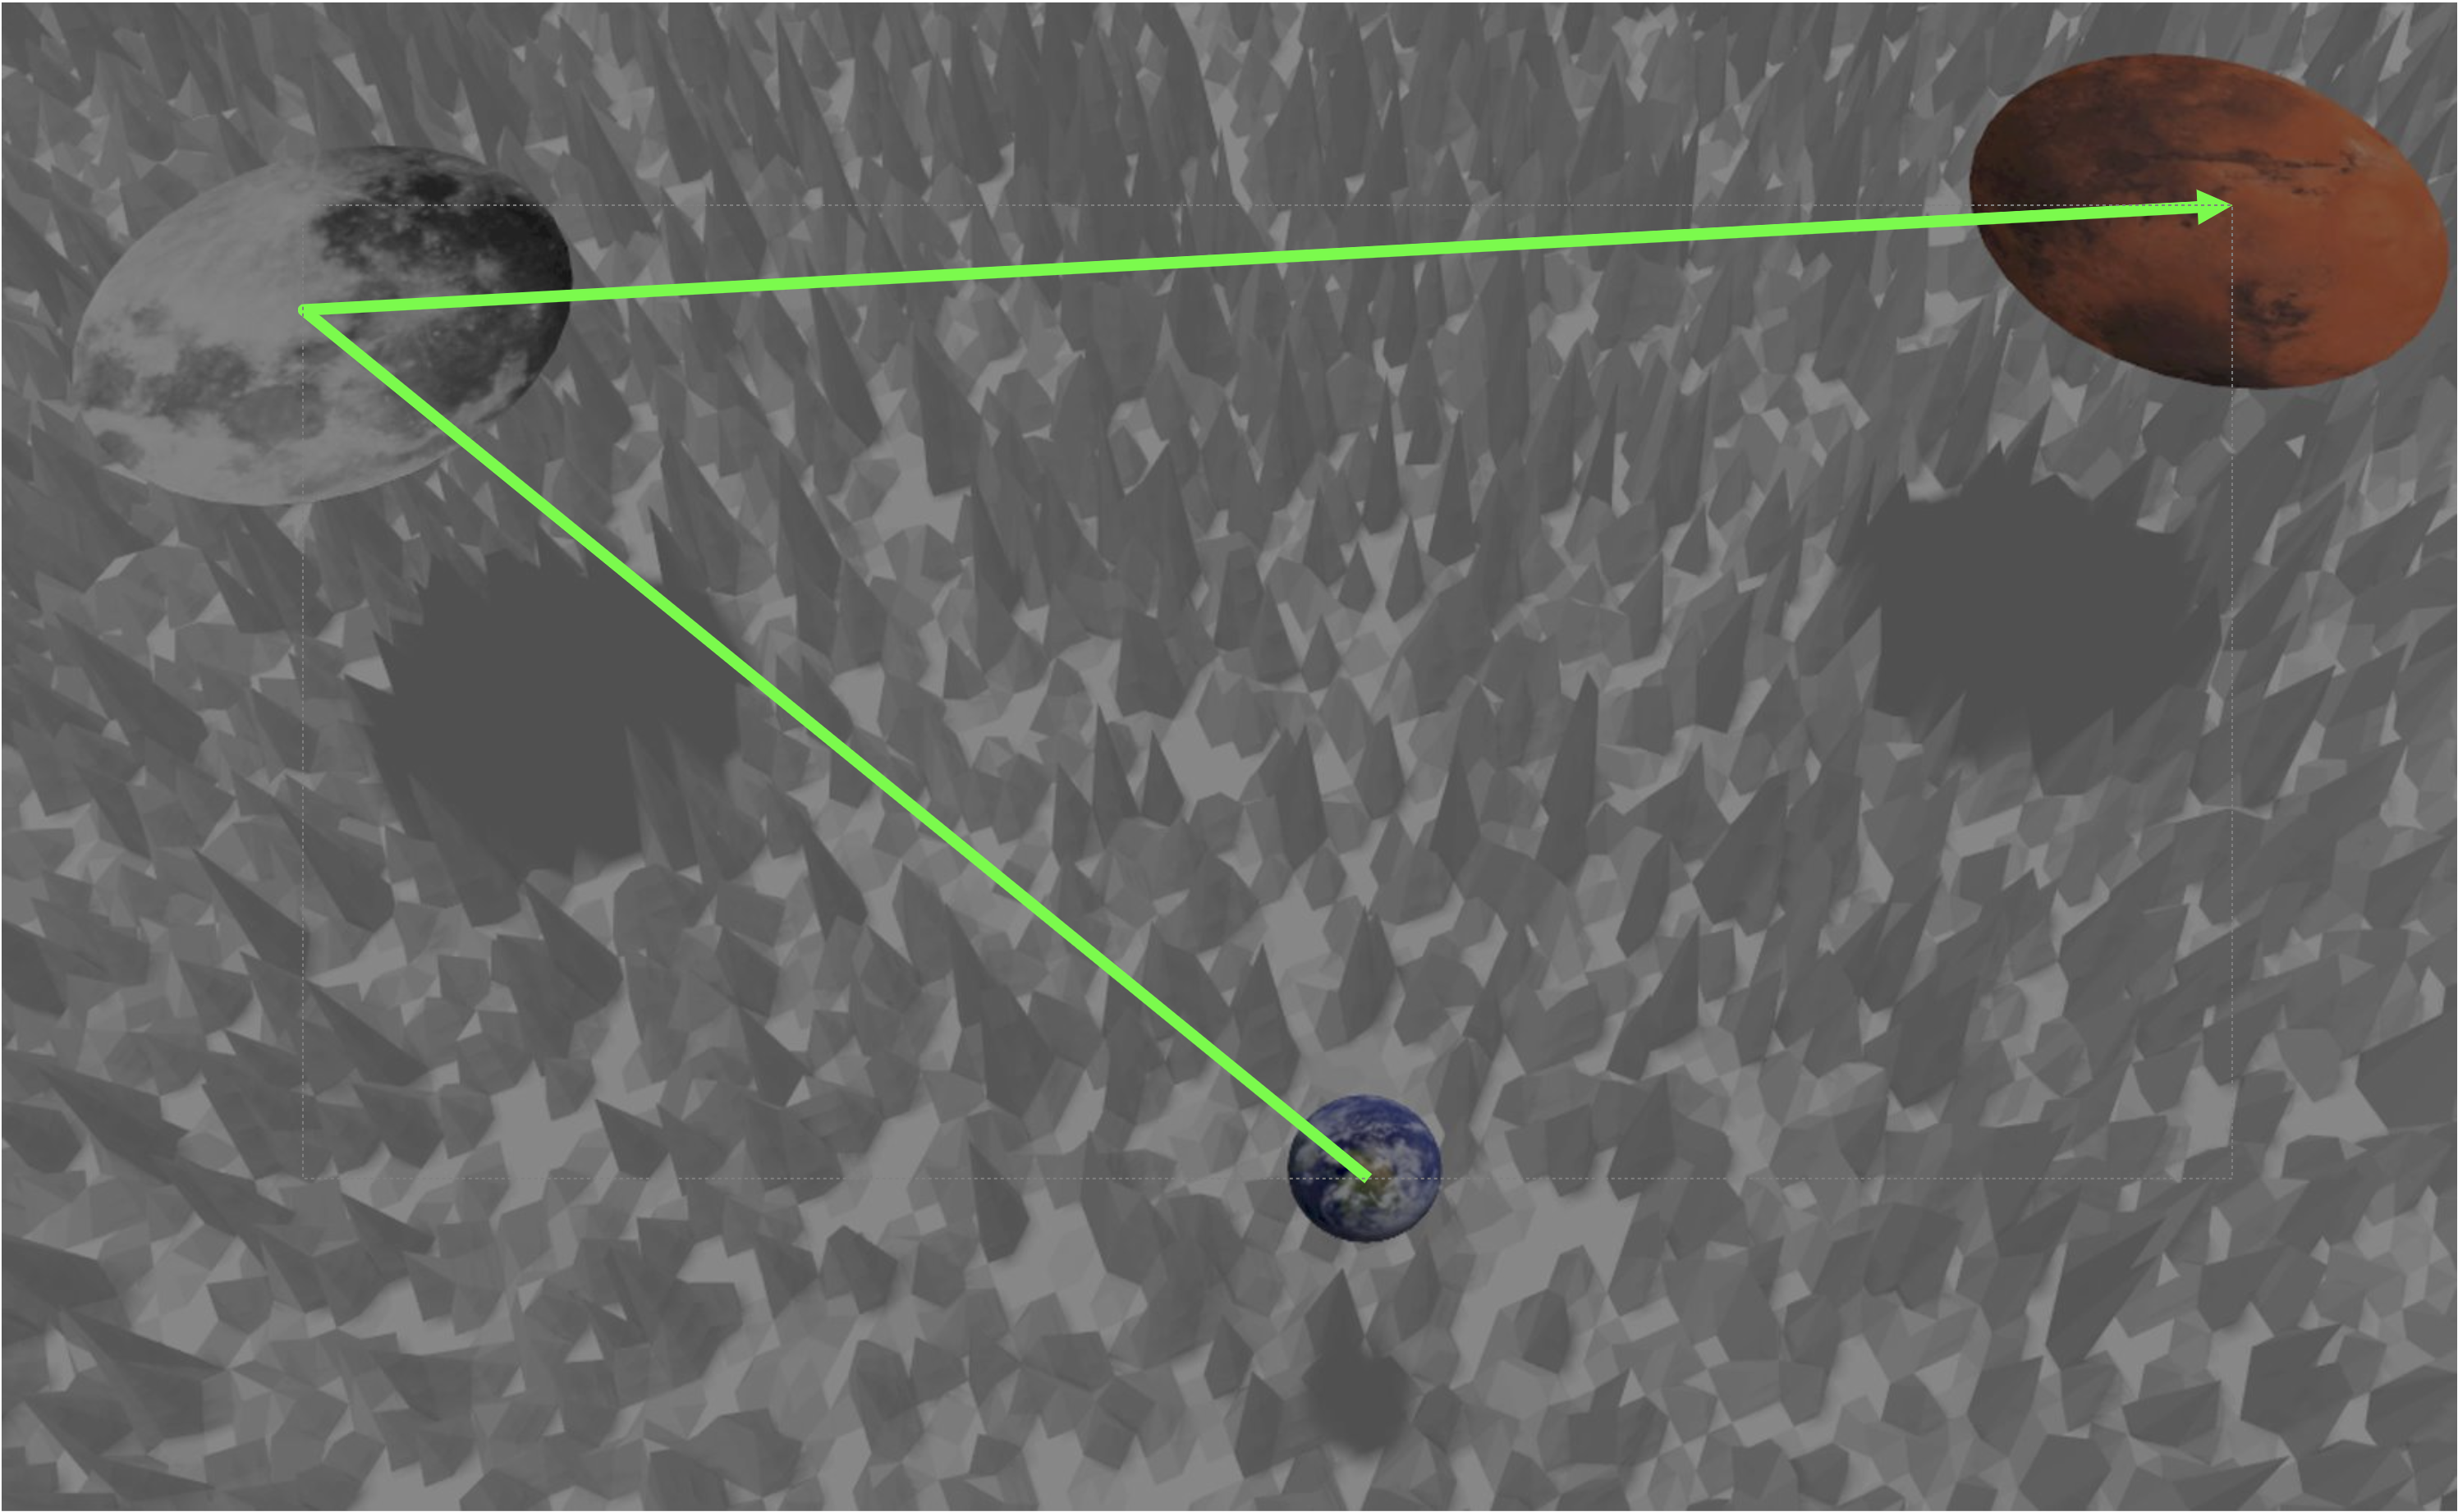
\includegraphics[scale=0.24]{images/evaluation/rough_over_platforms.png}
            \caption{Test flights on rough map with waypoints covering the landing sites}
            \label{fig:rough_covered}
        \end{figure}

        In this test, the drone flew a randomized two-waypoint pattern which always covered the synthetically added landing platforms. The idea behind this experiment was to eliminate other landing possibilities and test, whether the approach at hand would be able to detect the controlled good landing sites.

        The numerical result thereof is displayed below:

        \begin{table}[h]
            \begin{center}
             \caption{Results - Rough map with platform coverage}\vspace{1ex}
             \label{tab:result_rough_covered}
             \begin{tabular}{|c|c|c|c|c|}
             \hline
             \# Flights & \# Successes & \# Timeouts & \# Crashes & \# Home Landing\\ \hline \hline
             100 & 97 & 3 & 0 & 0 \\%TODO: replace with correct values
             \hline
             \end{tabular}
            \end{center}
        \end{table}

        \begin{table}[h]
            \begin{center}
             \caption{Landing attempts rough map with platform covering mission}\vspace{1ex}
             \label{tab:land_nums_rough_coverage}
             \begin{tabular}{|c|c|c|c|}
             \hline
             \# Flights & \# Landing on first attempt & \# 2 attempts & \# 3 attempts\\ \hline \hline
             100 & 50 & 47 & 3 \\%TODO: replace with correct values
             \hline
             \end{tabular}
            \end{center}
        \end{table}

        As for this test all landing sites are the randomly placed platforms, visualizing the landing attempt locations is useless.

        \subsubsection{Numerical Discussion}
        %TODO



    \subsection{Rough Map - Completely Random Waypoints}

    \begin{figure}[h]
        \centering
        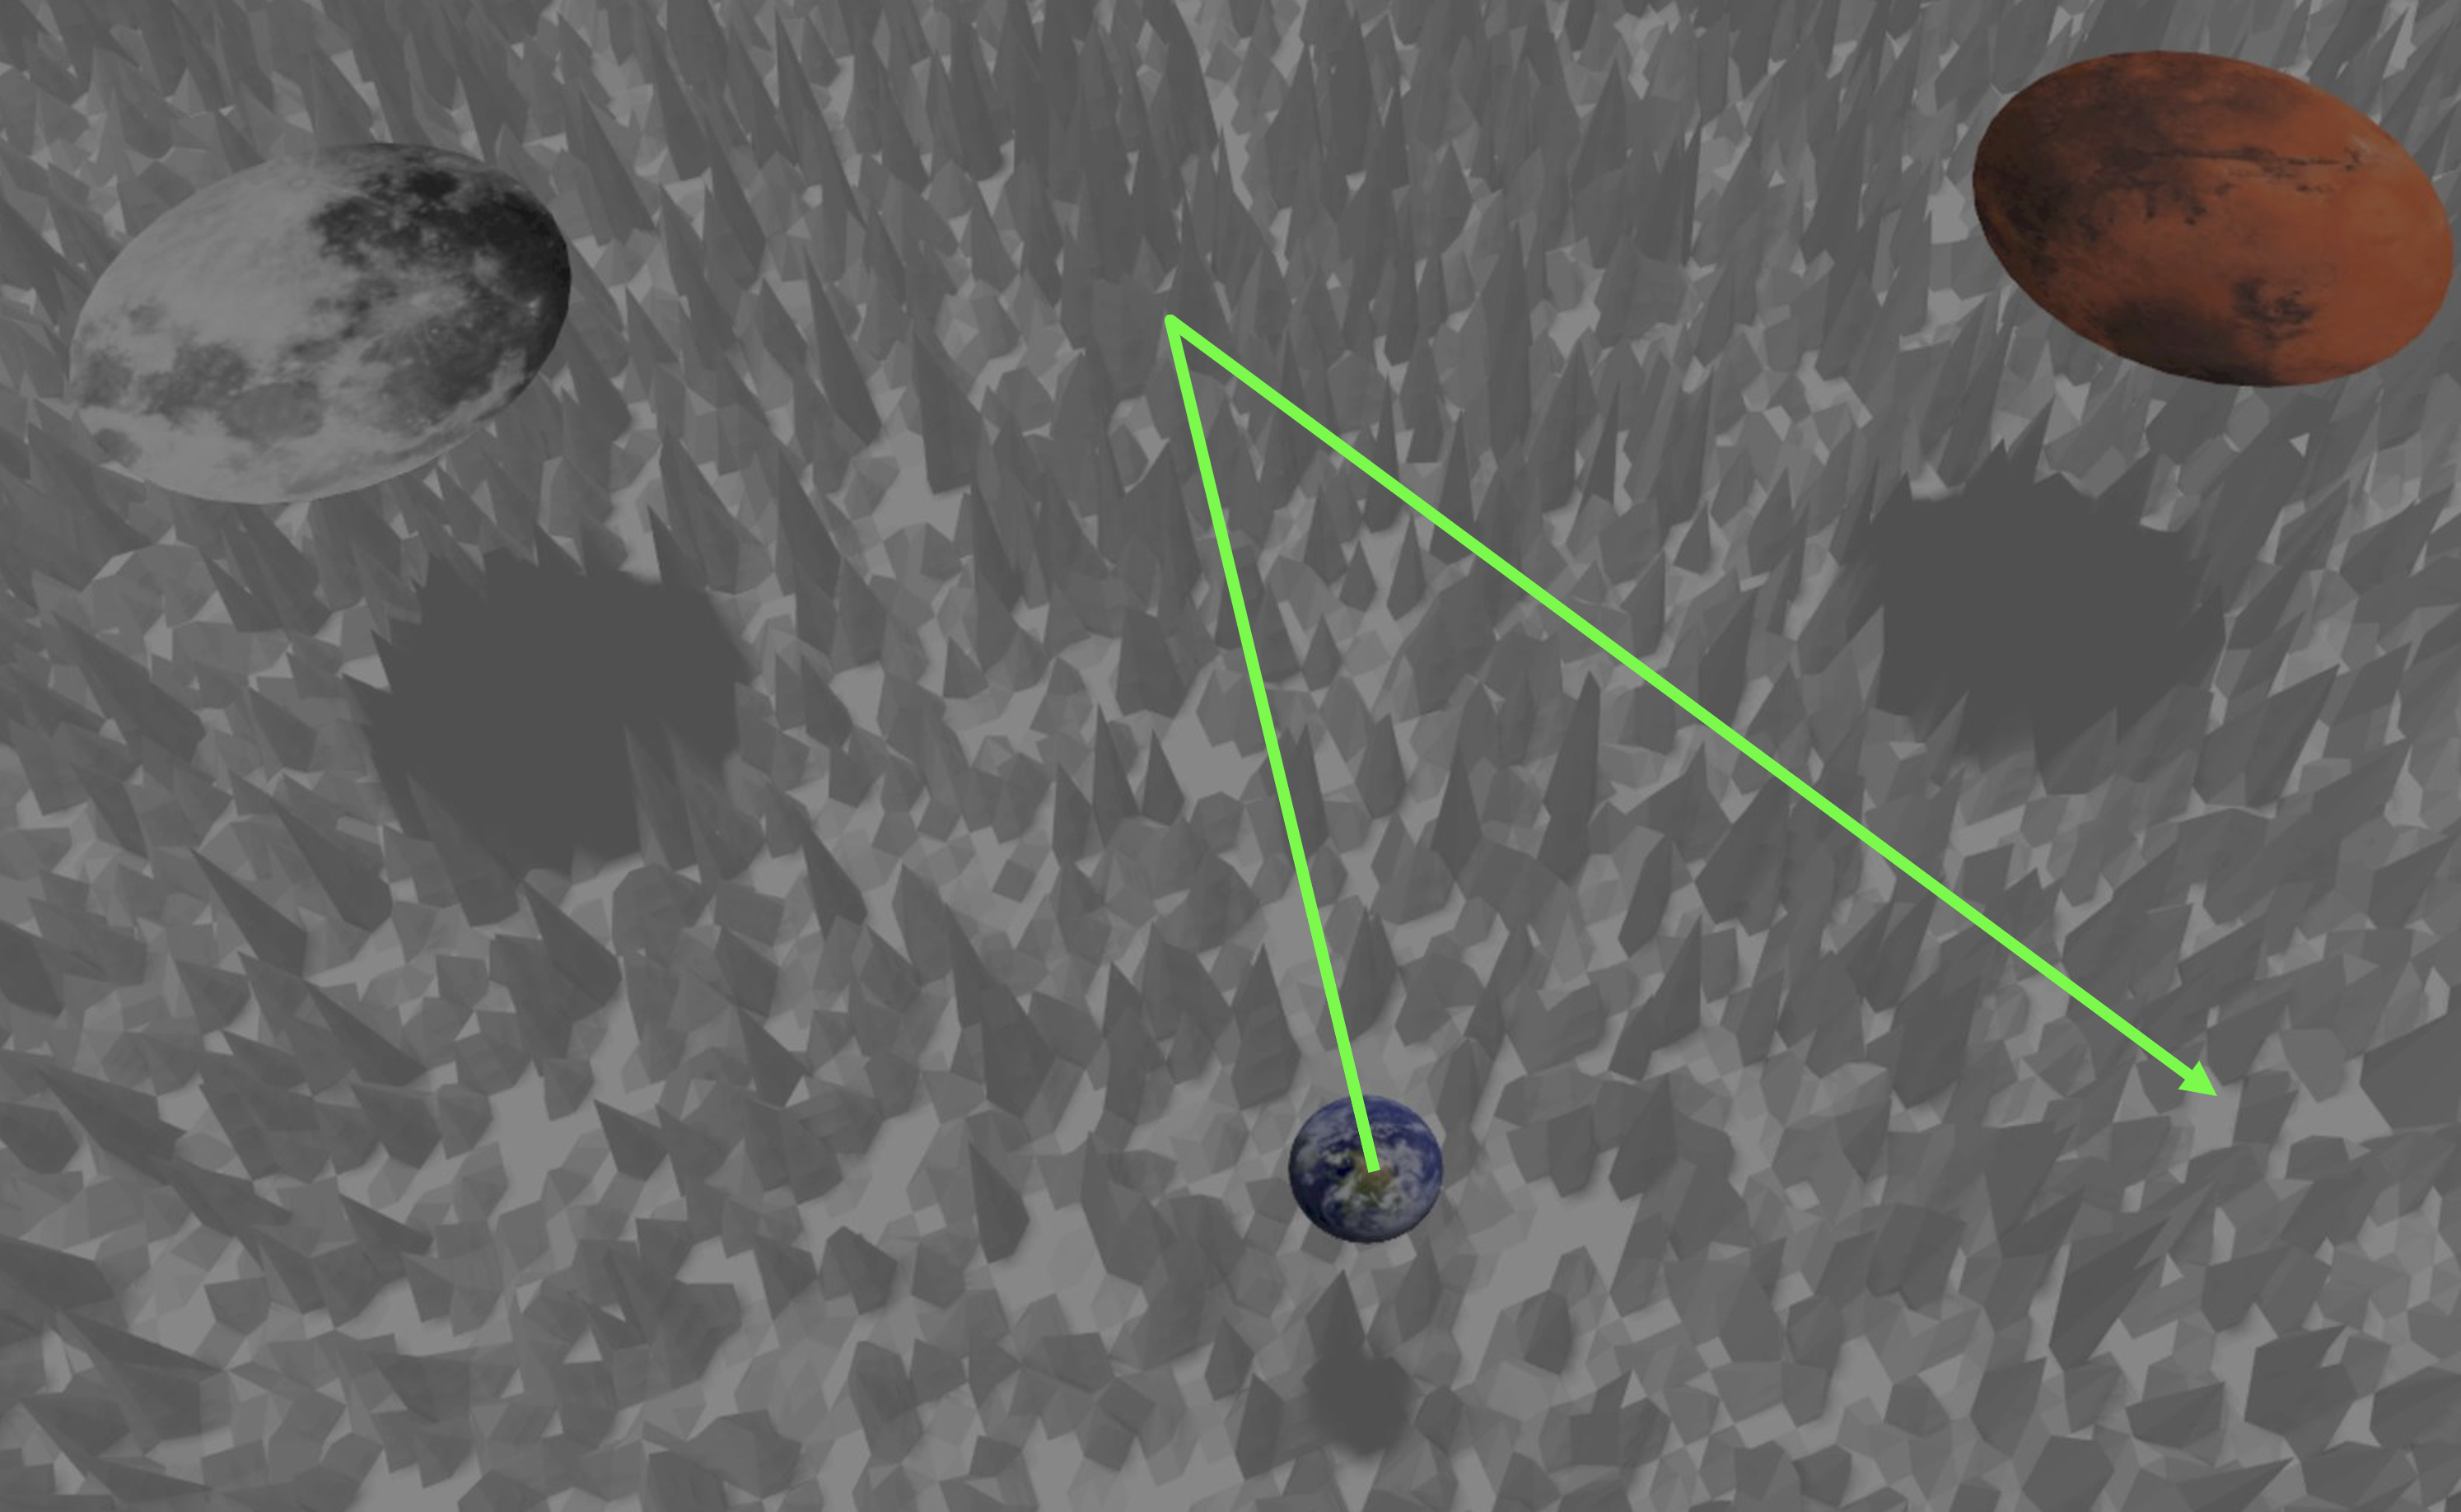
\includegraphics[scale=0.24]{images/evaluation/rough_complete_rand.png}
        \caption{Test flights on rough map with waypoints covering the landing sites}
        \label{fig:rough_compl_rand}
    \end{figure}

    In this test, the drone flew a completely randomized two-waypoint pattern. As very often the mission trajectory did not cover the spawned platforms, this test set analyzed the pipeline's capabilities to deal with the case when no landing sites are detected initially.

    The numerical result thereof is displayed below:

    \begin{table}[h]
        \begin{center}
         \caption{Results - Rough map with platform coverage}\vspace{1ex}
         \label{tab:result_rough_rand}
         \begin{tabular}{|c|c|c|c|c|}
         \hline
         \# Flights & \# Successes & \# Timeouts & \# Crashes & \# Home Landing\\ \hline \hline
         100 & 97 & 3 & 0 & 0 \\%TODO: replace with correct values
         \hline
         \end{tabular}
        \end{center}
    \end{table}

    \begin{table}[h]
        \begin{center}
         \caption{Landing attempts rough map without platform covering mission}\vspace{1ex}
         \label{tab:land_nums_rough_rand}
         \begin{tabular}{|c|c|c|c|}
         \hline
         \# Flights & \# Landing on first attempt & \# 2 attempts & \# 3 attempts\\ \hline \hline
         100 & 50 & 47 & 3 \\%TODO: replace with correct values
         \hline
         \end{tabular}
        \end{center}
    \end{table}

    Like in \cref{subsec:rough_coverage} there is no point in displaying the landing attempt locations.

    \subsubsection{Numerical Discussion}

    Notably, the drone went to the home position quite often. This is the desired behavior, when no landing site was found. %TODO analyze also how many lses were found using the additional patterns.
